\chapter{Results}

\section{Tire/road friction for different driving sessions}

\subsection{Winter tires on asphalt}

\begin{figure}[h]
	\centering
	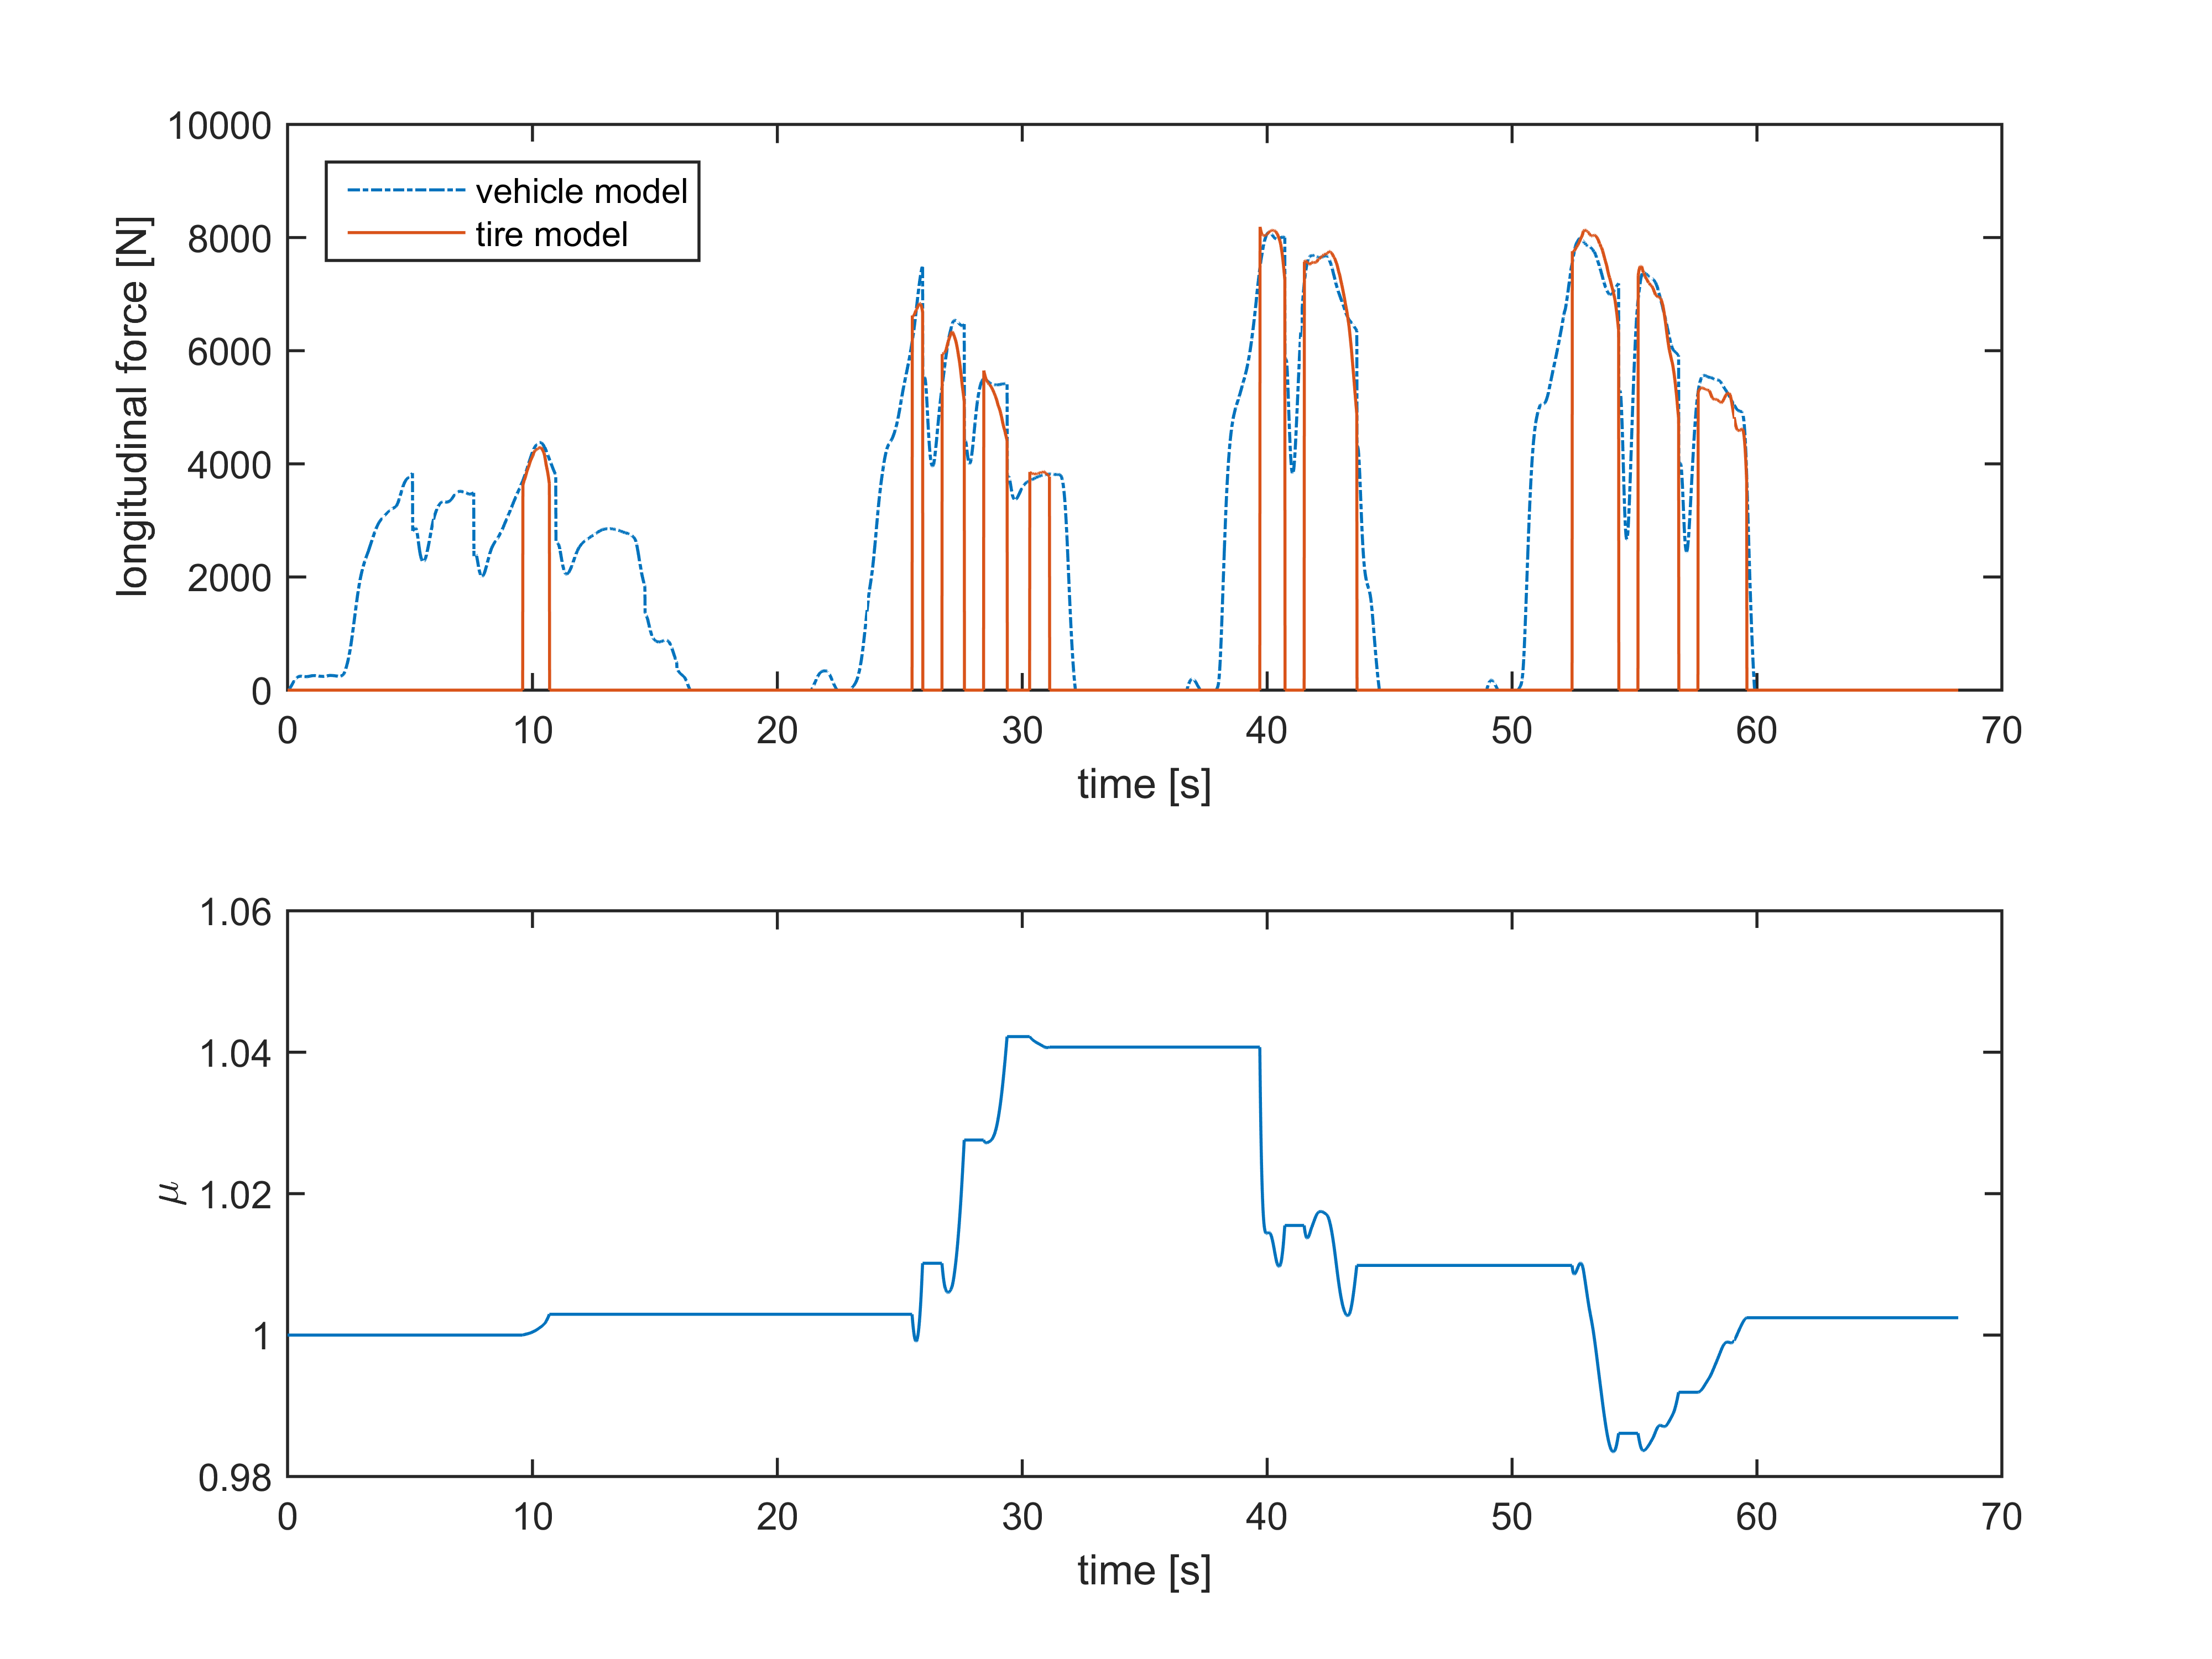
\includegraphics[width=1.0\textwidth]{Pictures/force_mue_olika_acc}
	\caption {Force from the tire and vehicle model and the approximated $ \mu $ for a straight line acceleration.}
	\label{force_mue_olika_acc}
\end{figure}

\begin{figure}[h]
	\centering
	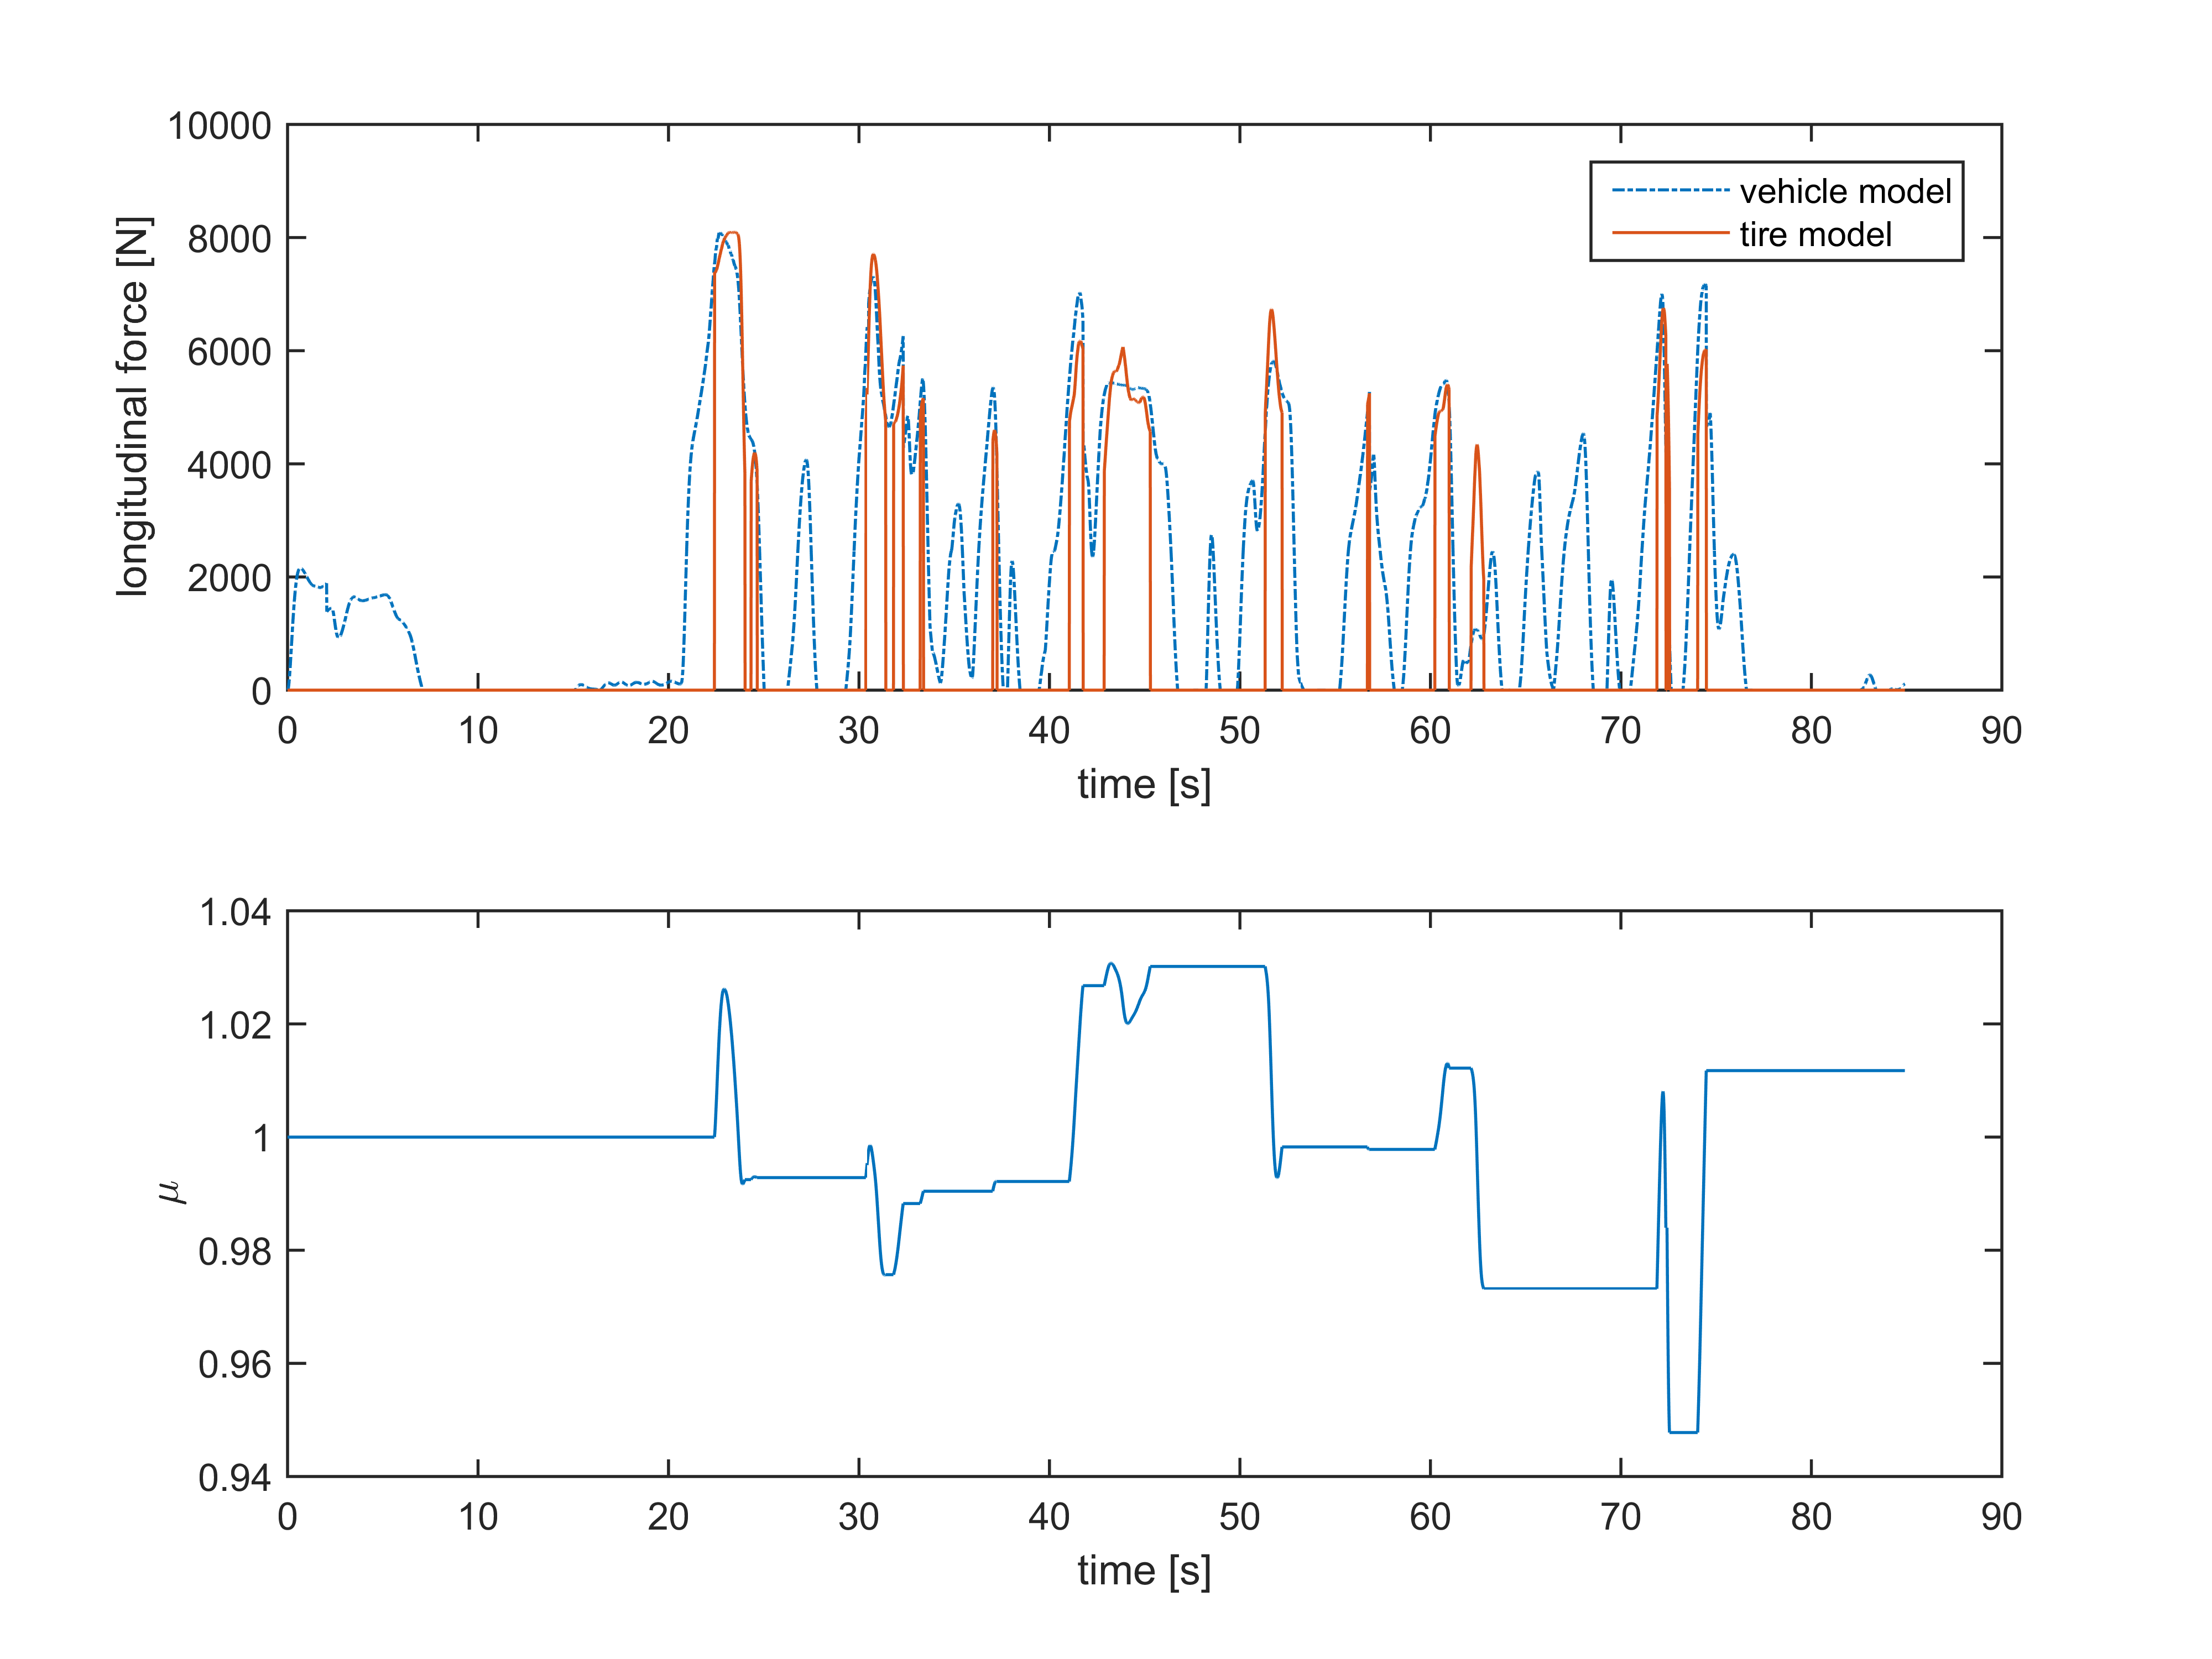
\includegraphics[width=1.0\textwidth]{Pictures/force_mue_race}
	\caption {Force from the tire and vehicle model and the approximated $ \mu $ for a fast track run.}
	\label{force_mue_race}
\end{figure}


\subsection{Winter tires on ice}

\begin{figure}[h]
	\centering
	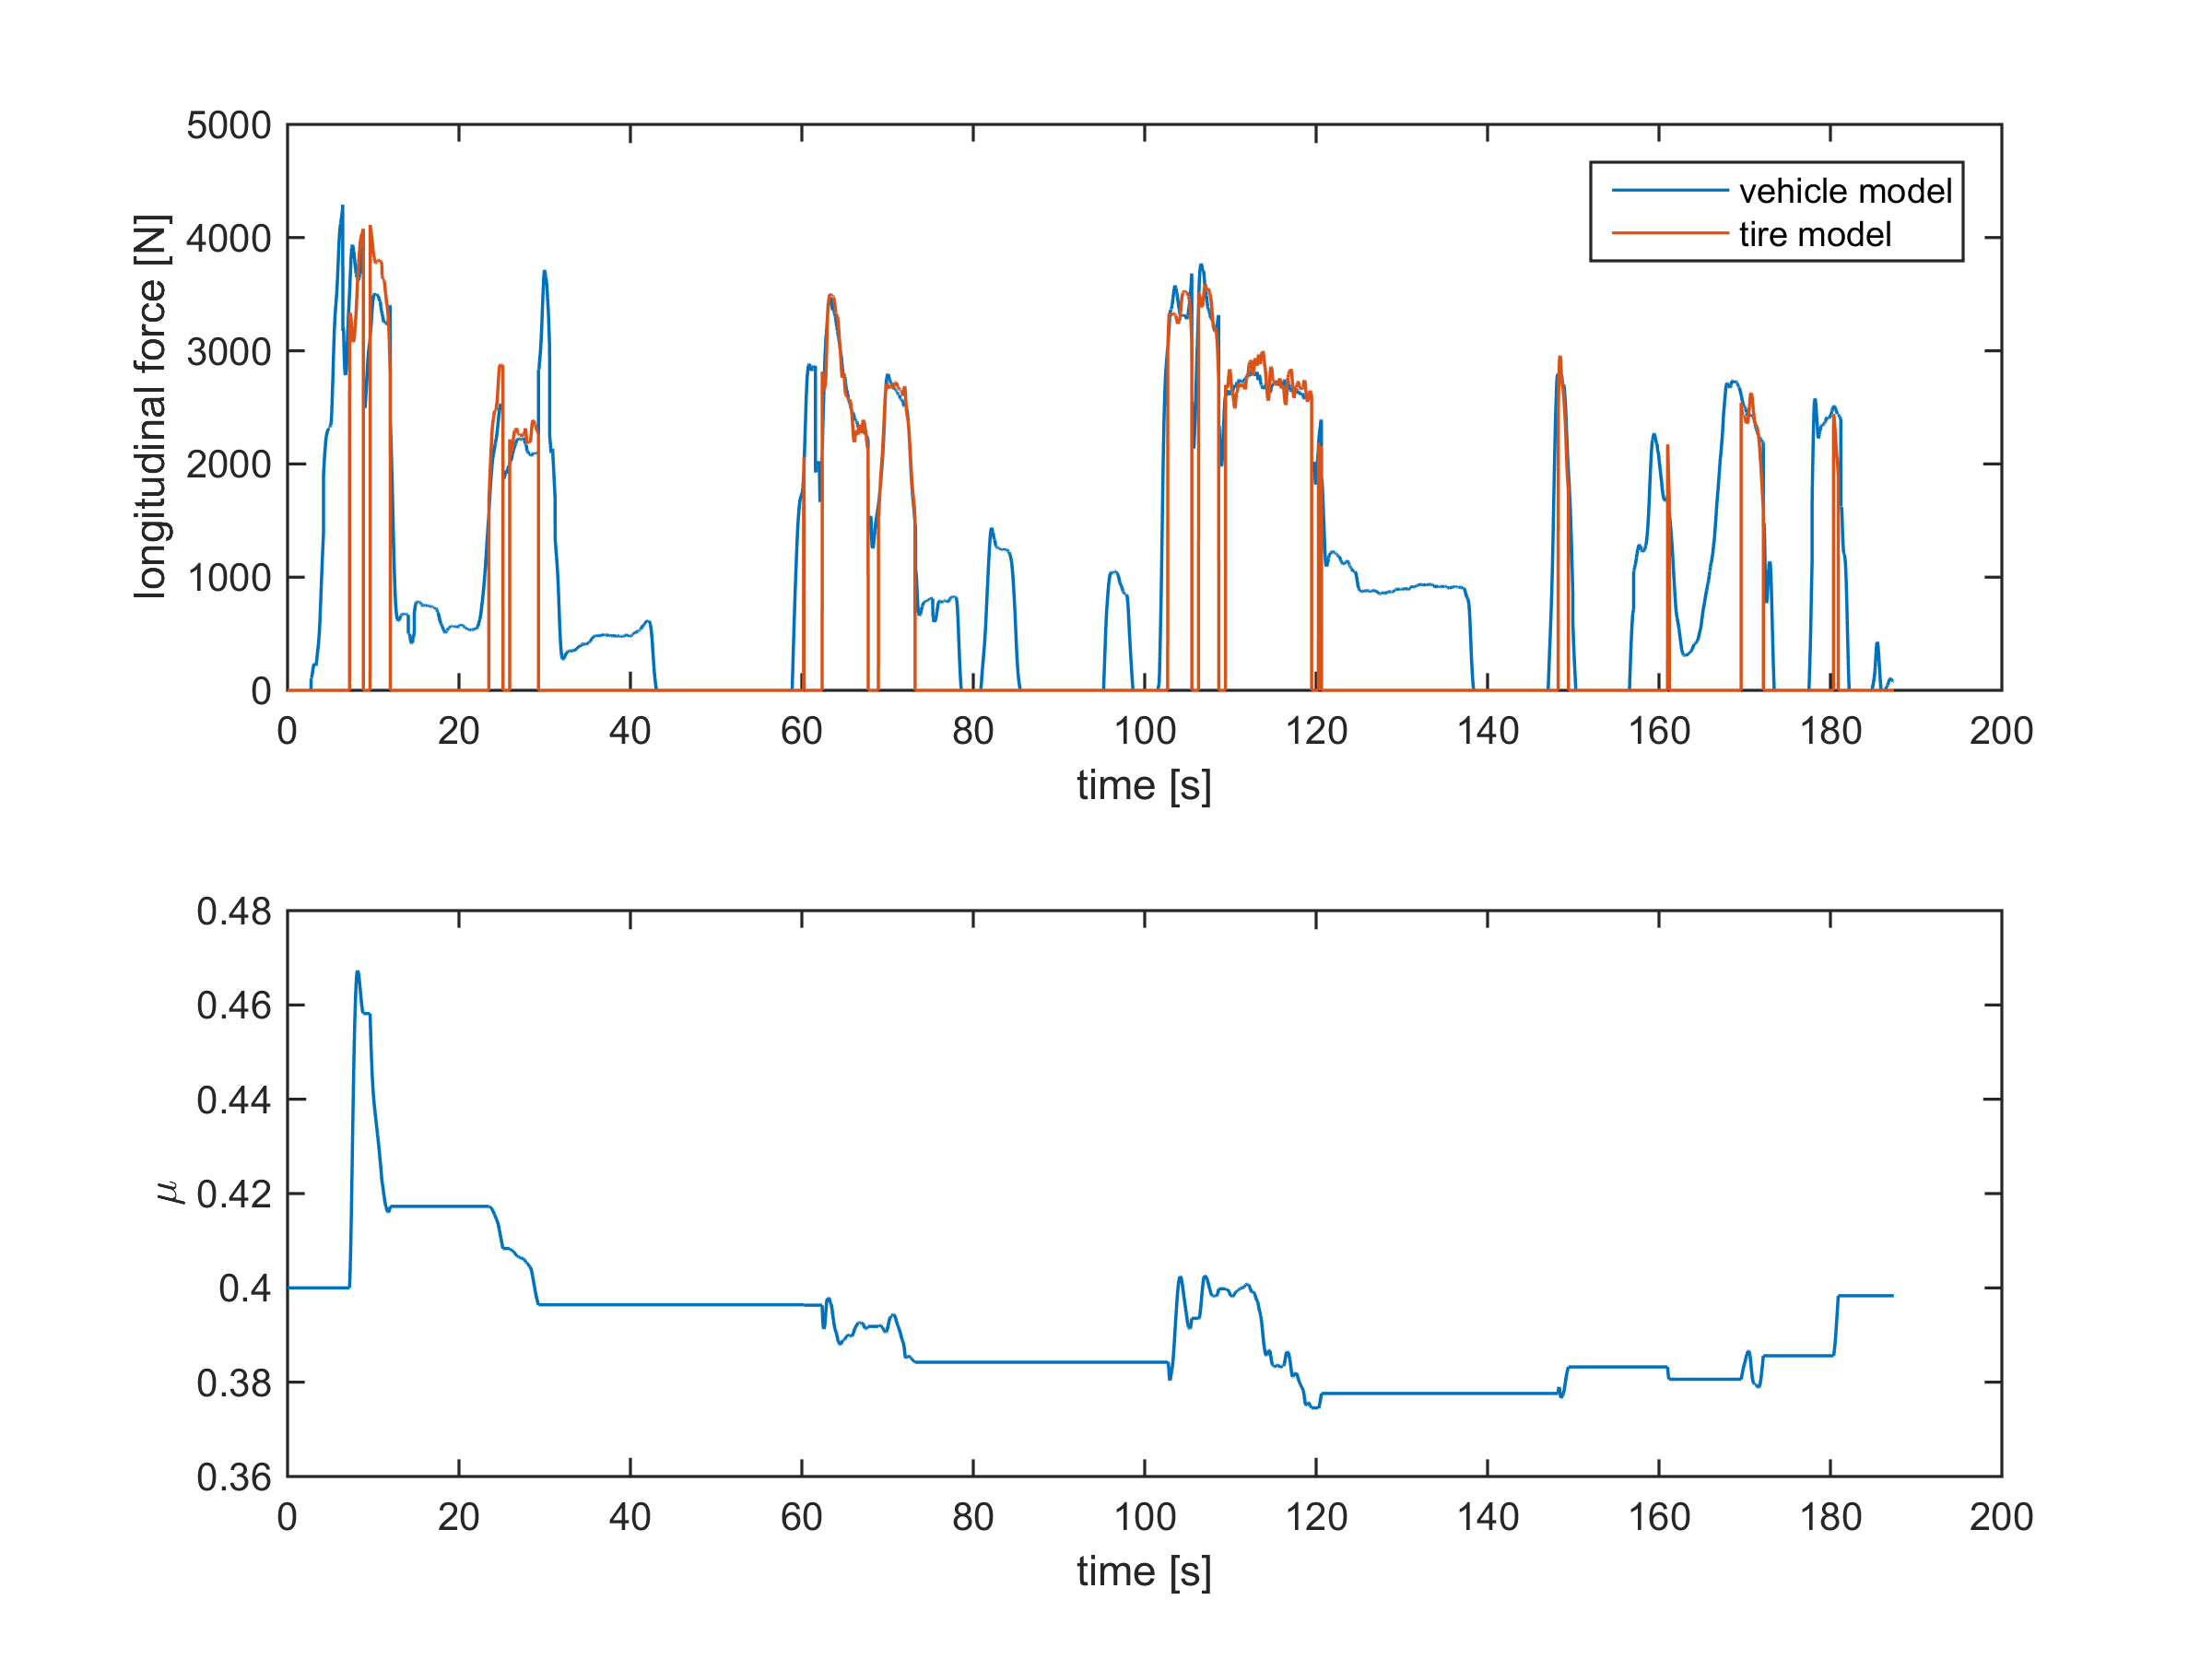
\includegraphics[width=1.0\textwidth]{Pictures/force_mue_ice_normal}
	\caption {Force from the tire and vehicle model and the approximated $ \mu $ for a fast track run.}
	\label{force_mue_ice_normal}
\end{figure}

\subsection{Winter tires on asphalt and ice combined}
The main goal for the work done in this report was to detect when low-$ \mu $ is present so that the torque transfer through the FXD can be limited. It is therefore essential to test the developed algorithm during a driving sequence that actually includes a changing $ \mu $. It has not been possible to test this on a single run, for example on asphalt and a skid pad. Therefore, two different runs have been merged together, where the friction coefficient changes three times.

The normalized force per slip ratio for this combined sequence can be seen in Figure \ref{slip_kraft_comb2}. Note that this figure is is merely Figure \ref{slip_kraft_ljungby} and \ref{slip_kraft_is} merged together, with some erroneous result when the friction coefficient changes come. 

\begin{figure}[h]
	\centering
	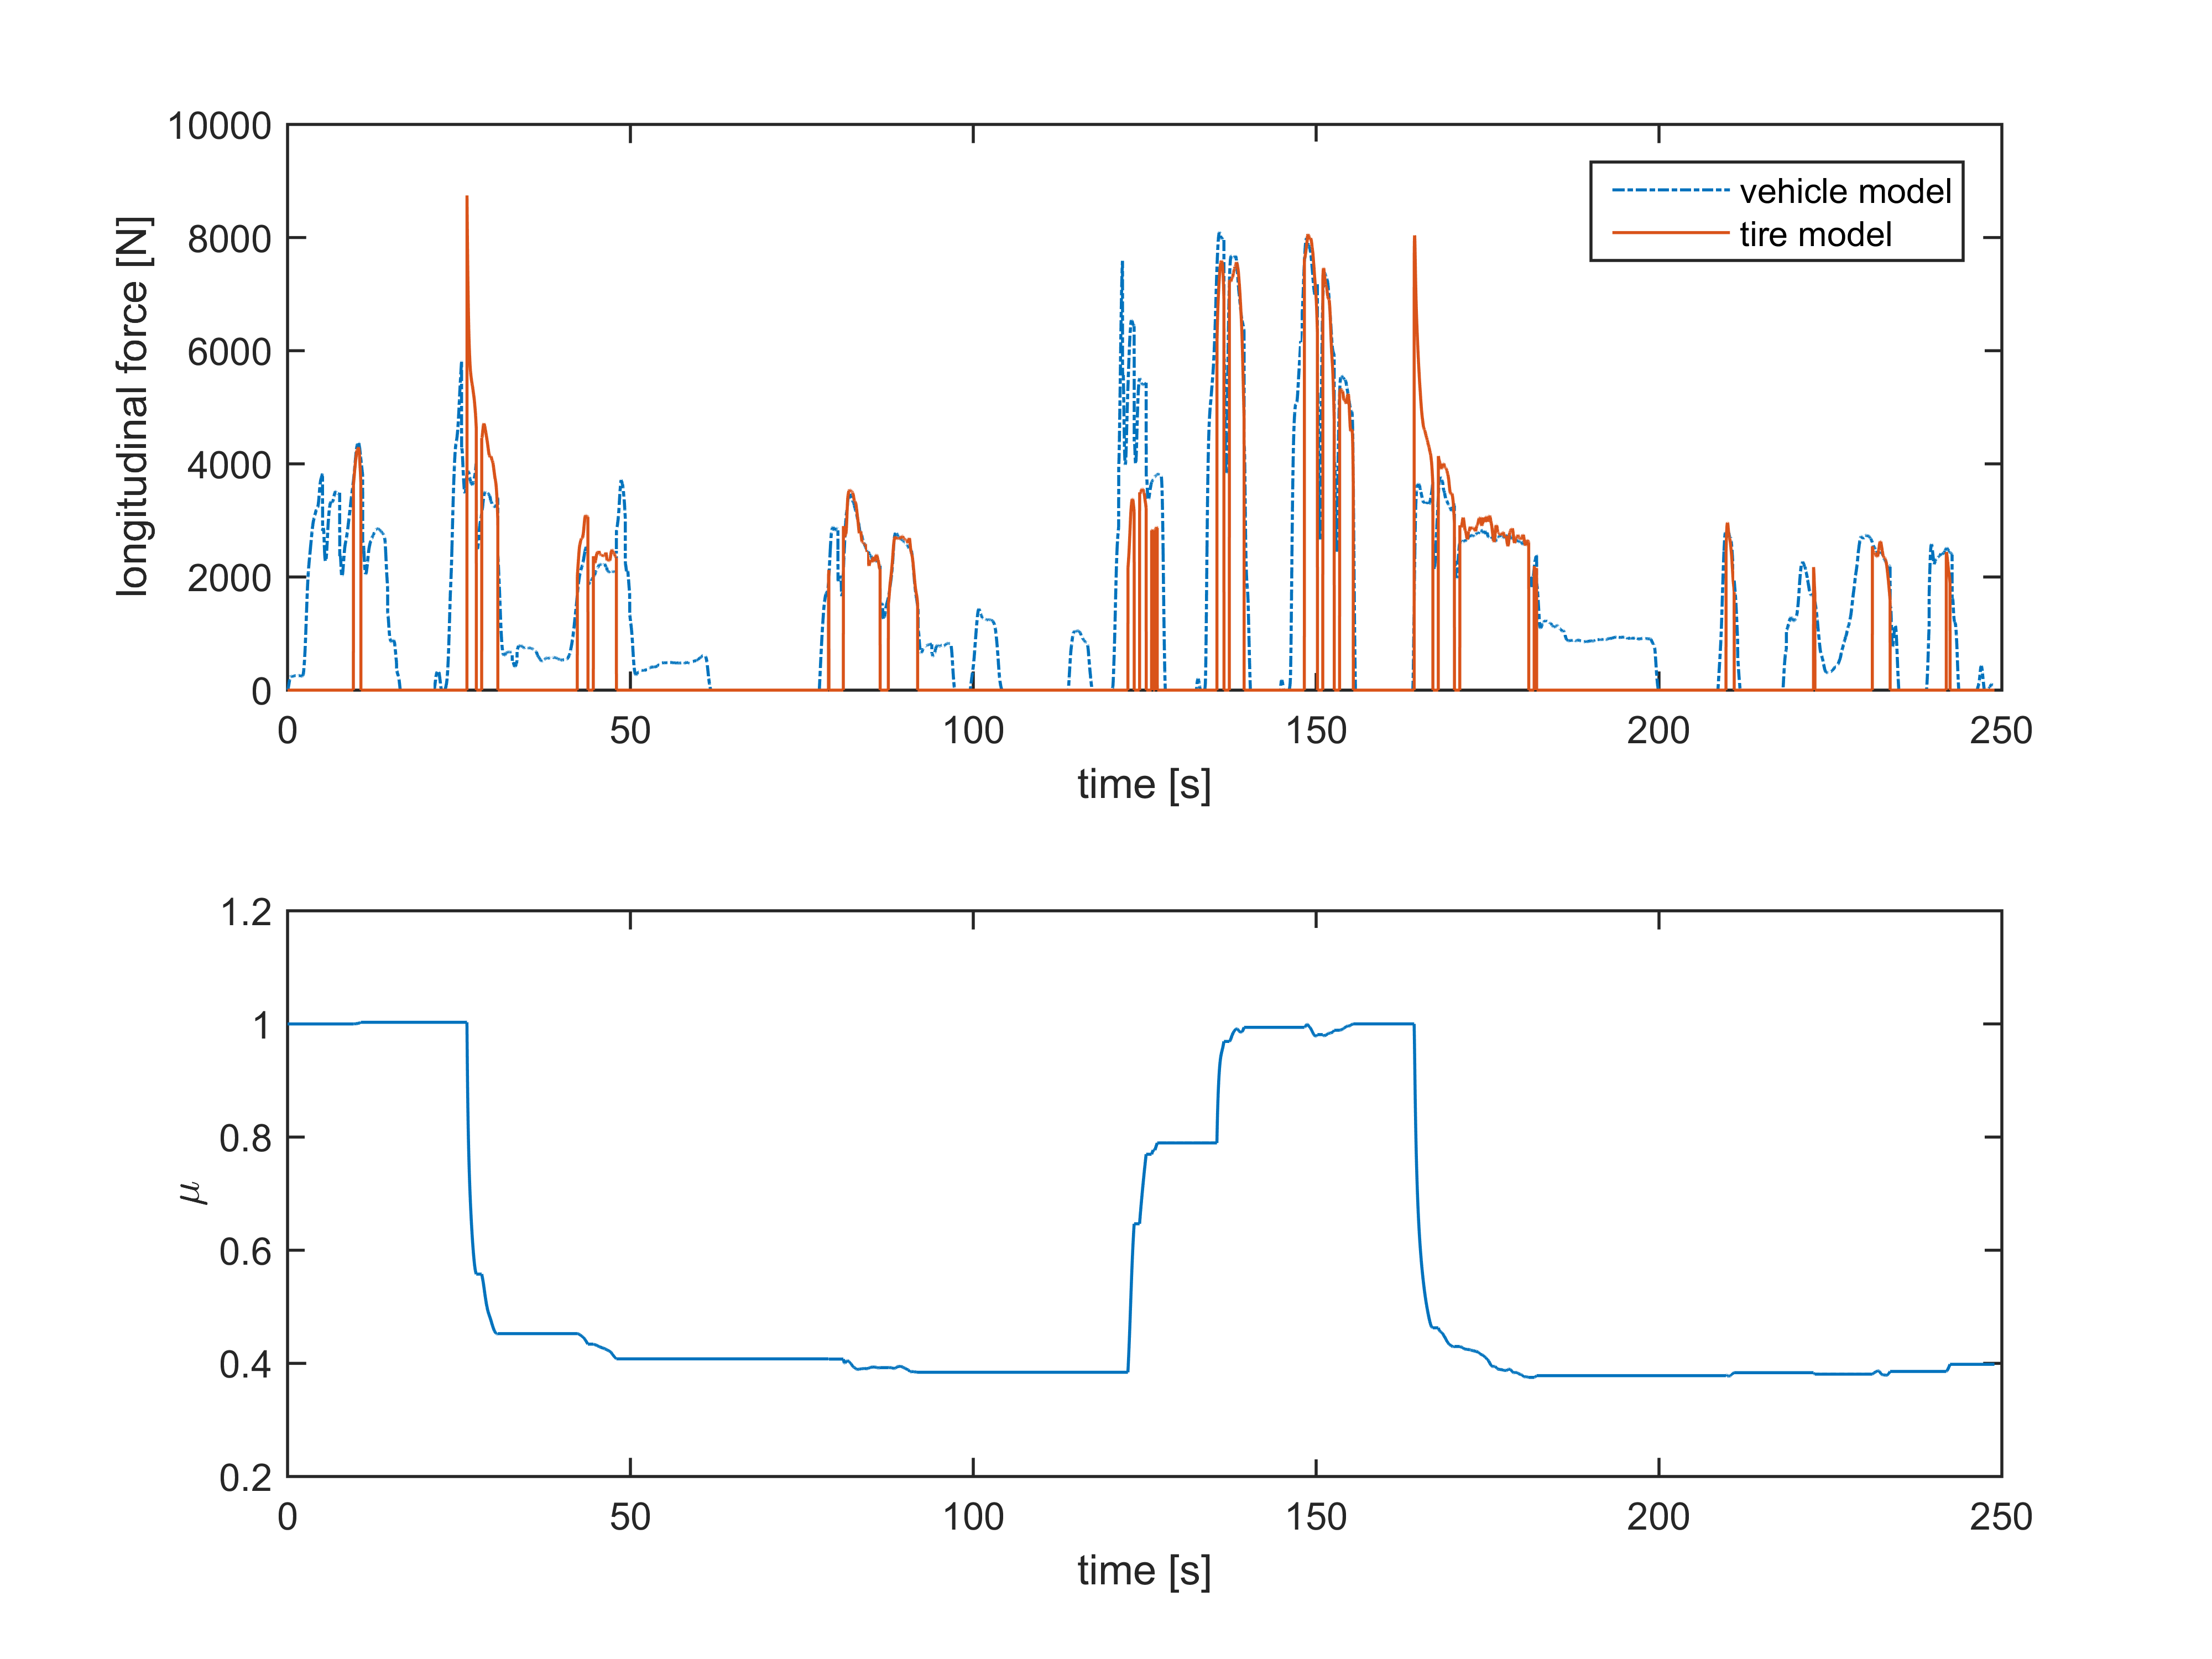
\includegraphics[width=1.0\textwidth]{Pictures/force_mue_comb2}
	\caption {Force from the tire and vehicle model and the approximated $ \mu $ for a fast track run.}
	\label{force_mue_comb2}
\end{figure}

\begin{figure}[h]
	\centering
	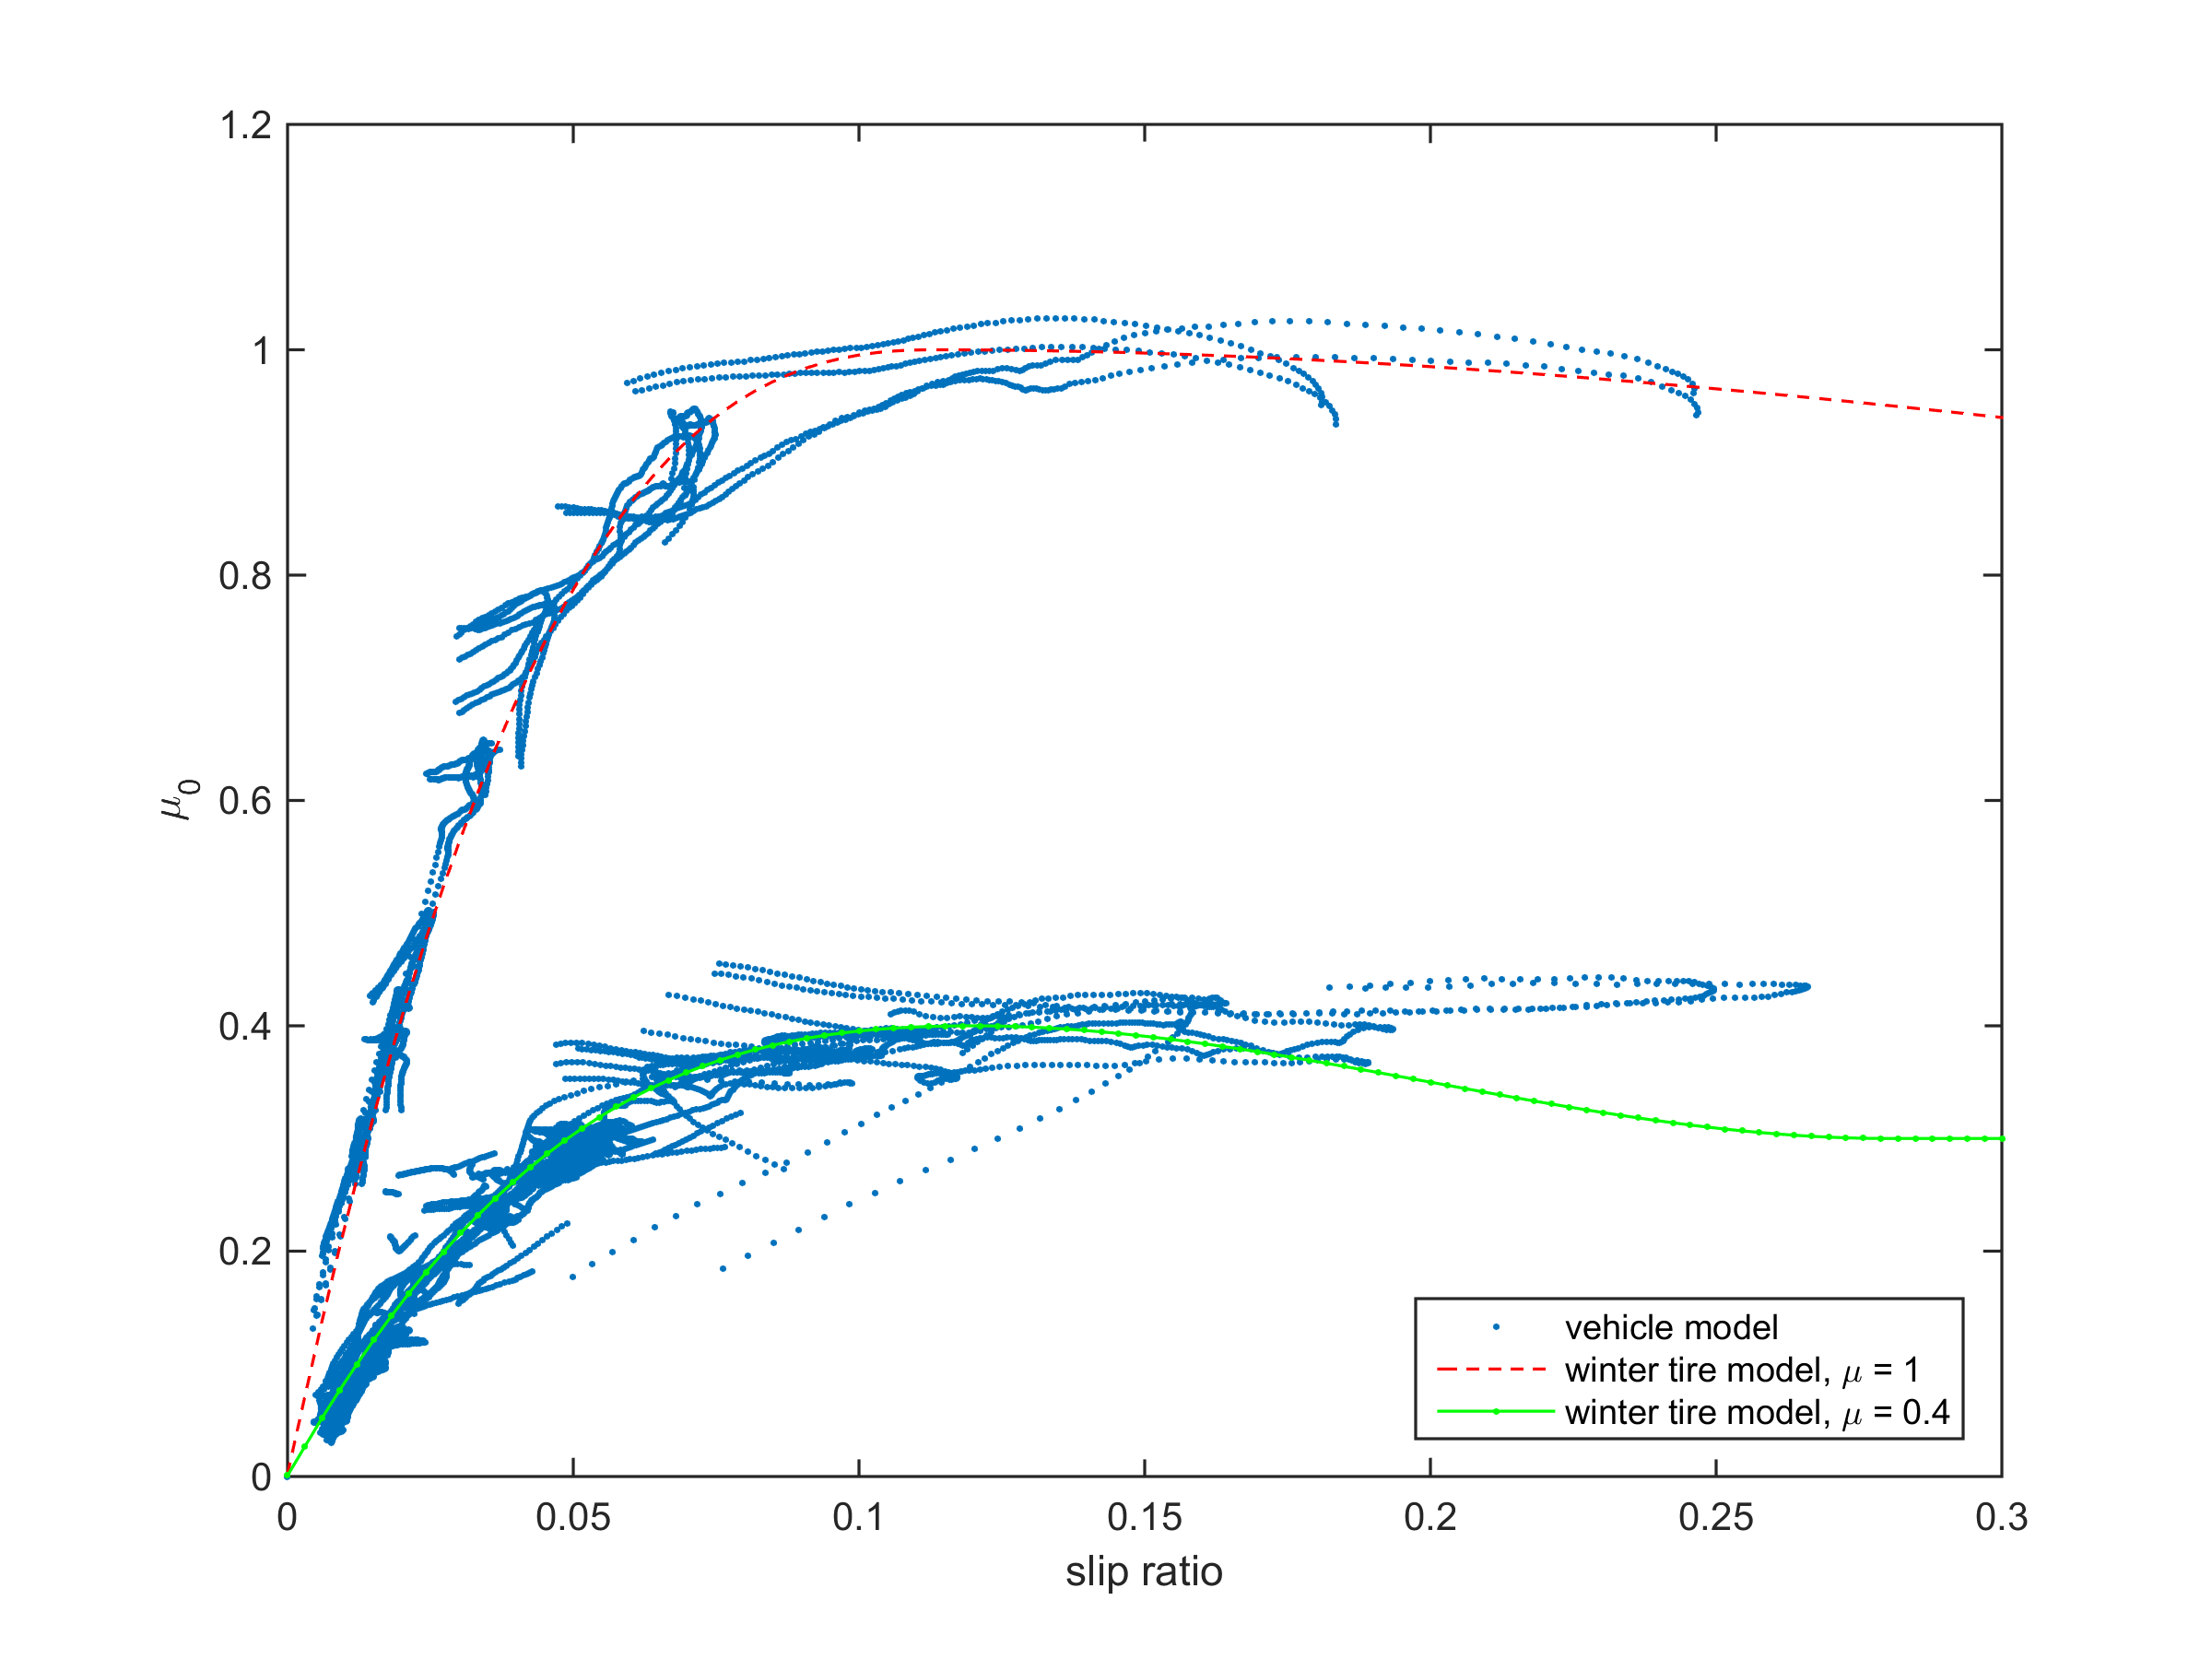
\includegraphics[width=1.0\textwidth]{Pictures/slip_kraft_comb2}
	\caption {Force per slip ratio for the combined driving sequence with both low- and high-$ \mu $.}
	\label{slip_kraft_comb2}
\end{figure}

\subsection{Summer tires on asphalt}

\subsection{Summer tires on wet asphalt}

\section{The used CAN signals}
Explain which signals are used throughout the report. Why are some not needed?.
